\section{Research Method} \label{sec:research_method}

{
\color{blue}
We used a multi-method approach to achieve our results. First, we used Grounded
Theory (GT) as the research method to build an explanation about how DevOps was
successfully adopted in companies that claims to have made it. Based on this
explanation, we proposed a model to guide new adopters. Finally, we used
Focus Group as method to explore in details a real experience on DevOps adoption,
including the application of our model.
}

\subsection{Grounded Theory}

We used Grounded Theory (GT) as the research method. GT was
originally proposed by Glaser and Strauss~\cite{glase1967discovery}.
As distinguishing features, GT has (1) the absence of clear research hypothesis upfront
and (2) limited exposure to the literature at the beginning of the research. GT
is a theory-development approach (the hypothesis emerge as a result of
a investigation), in contrast with more traditional
theory-testing approaches~\cite{coleman2007using}---e.g., those that
use statistical methods to either confirm or refute pre-established hypothesis.

We used GT as the research method is motivated due to three main reasons. First, GT is a consolidated
method in other areas of research --- notably medical
sociology~\cite{gt_medical_sociology}, nursing~\cite{barnsteiner2002using}, education~\cite{gt_education},
and management~\cite{gt_management}. More recently, GT is also being increasingly employed
to study software engineering research topics~\cite{hoda2017becoming,stol2016grounded,adolph2011using}. Second,
GT is considered an adequate approach to answer research questions that aims to
characterize scenarios under a personal perspective of those
engaged in a discipline or activity~\cite{barnsteiner2002using},
which is exactly the scenario here (i.e., what are the successful adoption paths for DevOps?). Finally,
GT allows researchers to build an independent and original understanding,
which is adequate to collect empirical evidence directly from the
practice on industry without bias of previous research. The evidence
is only reintegrated back with the existing literature after the step of
theory construction.

Since the publication of the original version of GT~\cite{glase1967discovery},
several modifications and variations have been proposed to the method, coming to
exist at least seven different versions~\cite{denzin2007grounded}.
Here we chose the classic version, mainly because we did not have a research
question at the beginning of our research, exactly as suggested in this
version. We actually started from an area of interest: successful DevOps adoption
in industry. In addition, research works in software engineering that leverage GT
predominantly use this version~\cite{stol2016grounded}.
We carried out our research using an existing
guideline about how to conduct a
Grounded Theory~\cite{adolph2011using} research. This guideline organizes
a GT investigation in 3 steps: \emph{Open Coding} Data Collection,
\emph{Selective Coding} Data Analysis, and \emph{Theoretical Coding}.

\begin{enumerate}[label=(\Alph*)]
\item {\bf Open Coding Data Collection.} We started our research
  by collecting and analyzing data from companies that claim to have
  successfully adopted DevOps.
  To this end, we have conducted a \emph{raw data analysis} that searches for patterns of
  incidents to indicate concepts,  and then grouped these concepts into
  categories~\cite{stol2016grounded}.

\item {\bf Selective Coding Data Analysis.} In the second step, we evolve
  the initial set of
  categories by comparing new incidents with the previous ones. Selective coding
  starts when a ``core category'' is identified~\cite{stol2016grounded}.
  The core category is responsible for enabling the integration of the other
  categories and structuring the results into a dense and consolidated grounded
  theory~\cite{jantunen2014using}. In selective coding, we only considered the
  specific variables that are directly related to the core category, in order to
  enable the production of an harmonic theory~\cite{coleman2007using,hoda2011impact}.
  Selective coding ends when we achieve a theoretical saturation, which occurs
  when the last few participants provided more evidence and examples but no new
  concepts or categories~\cite{glase1967discovery}.

\item {\bf Theoretical Coding.} After saturation, we built a theory that
explains the categories and the relationships between the categories.
Additionally, we reintegrated our theory with the existing literature, which allowed us to compare our proposal
 with other theories about DevOps. That is, using a Grounded Theory approach,
 one should only conduct a literature review in later stages of a research,
in order to avoid external influences to conceive a theory~\cite{adolph2012reconciling}.

\end{enumerate}

Throughout the process, we wrote memos capturing thoughts and analytic
processes; the memos support the emerging concepts, categories, and their
relationships~\cite{adolph2012reconciling}.

Regarding data collection, we conducted semi-structured interviews with 15 practitioners of companies from
Brazil, Ireland, Portugal, Spain, and United States that
contributed to DevOps adoption processes in their companies. Participants
were recruited by using two approaches: (1) through direct contact in a \emph{DevOpsDays}
event in Brazil and (2) through general
calls for participation posted on DevOps user groups, social networks,
and local communities. In order to achieve a heterogeneous perspective
and increase the wealth of information in the results,
we consulted practitioners from a variety of companies.
Table~\ref{participant_table} presents the characteristics of the participants
that accepted our invitation.
To maintain anonymity, in conformance with the human ethics guidelines\gnote{REF},
hereafter we will refer to the participants as P1--P15 (first column). \emph{We
assumed a non-disclosure agreement with the investigated companies to use the
data only in the context of our study and, therefore, we cannot disclose them}.

\begin{table}[h!]
\centering
\caption{Participant Profile. SX means software development experience in years,
DX means DevOps experience in years, CN means country of work, and CS means
company size (S\textless100; M\textless1000; L\textless5000; XL\textgreater5000).}
\label{participant_table}

\begin{tabular}{p{0.5cm}p{4cm}p{0.4cm}p{0.45cm}p{0.5cm}p{1.8cm}p{0.3cm}} \toprule \centering
\textbf{P\#}          & \textbf{Job Title}
       & \textbf{SX} & \textbf{DX} & \textbf{CN}   & \textbf{Domain}    & \multicolumn{1}{l}{\textbf{CS}} \\ \midrule \centering
P1                   & DevOps Developer      & 9            & 2           & IR            & IT                 & S                               \\ \centering

P2                   & DevOps Consultant       & 9            & 3           & BR            & IT                 & M                               \\ \centering

P3                   & DevOps Developer      & 8            & 1           & IR            & IT                 & S                               \\ \centering

P4                   & Computer Technician        & 10           & 2           & BR            & Health             & S                               \\ \centering

P5                   & Systems Engineer      & 10           & 3           & SP            & Telecom            & XL                              \\ \centering

P6                   & Developer             & 3            & 1           & PO            & IT                 & S                               \\ \centering

P7                   & Support Analyst       & 15           & 2           & BR            & Telecom            & L                               \\ \centering

P8                   & DevOps Engineer       & 20           & 9           & BR            & Marketing              & M                               \\ \centering

P9                   & IT Manager            & 14           & 8           & BR            & IT                 & M                               \\ \centering

P10                  & Network Admin.        & 15           & 3           & BR            & IT                 & S                               \\ \centering

P11                  & DevOps Supervisor                & 6            & 4           & BR            & IT                  & M                               \\ \centering

P12                  & Cloud Engineer              & 9            & 3           & US            & IT                  & L                               \\ \centering

P13                  & Technology Manager                 & 18            & 6           & BR            & Food                  & M                               \\ \centering

P14                  & IT Manager            & 7            & 2           & BR            & IT                  & S                               \\ \centering

P15                  & Developer        & 3            & 2           & BR            & IT                  & S \\ \bottomrule
\end{tabular}
\end{table}



The interviews were conducted between April 2017 and April 2018 by means of Skype calls.
The interviews lasted a minimum of 20 minutes, a maximum of 50 minutes, and an average of 31 minutes.
Data collection and analysis were iterative so the collected data helped to guide
future interviews. Questions evolved according to
the progress of the research. We started with five open-ended questions: (1) What
motivated the adoption of DevOps? (2) What does DevOps adoption mean in the context of
your company? (3) How was DevOps adopted in your company? (4) What were the
results of adopting DevOps? And (5) what were the main difficulties?

As the analyzes were being carried out, new questions were added to the script.
These new questions were related to the concepts and categories identified in
previous interviews. Examples of new questions include: (1) What is the
relationship between deployment automation and DevOps adoption? (2) Is it
possible to adopt DevOps without automation? (3) How has your company fostered a
collaborative culture?

With respect to \emph{data analysis}, the interviews were
recorded, transcribed, and analyzed. The interviews with participants from
Brazil and Portugal were translated from Portuguese into
English. The first moment of the analysis, called open coding in GT, starts
immediately after the transcription of the first interview.
Open coding lasted until there was no
doubt about the core category of the study. Similar to that described by
Adolph et al.~\cite{adolph2012reconciling}, we started
considering a core category candidate and changed later. The first core category
candidate was \cat{automation}, but we realized that this category did not
explain most of the behaviors or events in data. The sense of
shared responsibilities in solving problems, and the notion of product thinking
are examples of events that could not be naturally explained in terms of \cat{automation}.
We then started to understand that \cc also appeared recurrently in the analysis
and with more potential to explain the remaining events. Thus, we asked the
respondents explicitly about the role of \cat{automation} and how the \cc is
formed in a DevOps adoption process.

Considering the script adaptations and the analysis of new data in a constant
comparison process, taking into account the previous analyses and the
respective memos written during all the process, after the tenth
interview, we concluded that \cc was the core
category regarding how DevOps was successfully adopted.
At this moment, the open coded ended and the selective coding started.
We started by restricting the coding only
to specific variables that were directly related to the core category and their
relationships. Following three more interviews and respective analysis, we realized that
the new data added less and less content to the emerging theory. That is, the
explanation around how the \cc category is developed showed signs of saturation.
We then conducted two more interviews to conclude that we had reached a
theoretical saturation, that is, we were convinced there were no more enablers
or outcomes related to DevOps adoption, the relationship between all of them
was adequate and the properties of core category were well developed.

{
\color{blue}
It is important to note that theoretical saturation is closely related to the
questions that one intends to answer in the collection and analysis of the data.
New questions can be asked and new aspects can be studied, demanding new rounds
of iterative data collection and analysis in search of the theoretical
saturation regarding that new aspect.
}

At this point, we started the theoretical coding to find a way to integrate
all the concepts, categories, and memos in the form of a cohesive and
homogeneous theory, where we have pointed out the role of the categories as
enablers and outcomes. We will present more details about
the results of our theoretical coding phase in the next section.
To illustrate the coding procedures, we will show a working example from an
interview transcription to a category.
It is important to note that \emph{raw interview transcripts} are full of noise.
We started the coding by removing this noise and identifying the key points.
Key points are summarized points from sections of the interview~\cite{georgieva2008best}.
For example:

\textbf{Raw data:} \textit{``So, here we have adopted this type of strategy that is
the infrastructure as code, consequently we have the versioning of our entire
infrastructure in a common language, in such a way that any person, a
developer, an architect, the operations guy, or even the manager, he can look
at it and describe that the configuration of application x is y. So, it
aggregates too much value for us exactly with more transparency''}

\textbf{Key point:} \textit{``Infrastructure as code contributes to
transparency because it enables the infrastructure versioning in a common
language to all professionals''}

We then assigned codes to the key point. A code is a phrase that summarizes
the key point and one key point can lead to several codes \cite{hoda2017becoming}.

\textbf{Code:} \textit{Infrastructure as code contributes to transparency}

\textbf{Code:} \textit{Infrastructure as code provides a common language}

In this example, the concept that emerged was ``infrastructure as code''. The
expression corresponding to this concept comes directly from raw data, but this
is not a rule. It is common for the concept to be an abstraction, without
emerging from an expression present in raw data.
At this moment, we already identified other concepts that
contribute to transparency. We wrote the following memo:

\textbf{Memo:} \textit{Similar to sharing on a regular basis and shared
pipelines, the concept of infrastructure as code is an important transparency
related one. These transparency related concepts have often been cited as
means to achieve greater collaboration between teams}.

The constant comparison method was repeated on the concepts to produce a third
level of abstraction called categories. Infrastructure as code was grouped
together with five other concepts into the \textbf{sharing and transparency} category.
Figure~\ref{fig1} illustrates how that abstraction of concepts become a category.


\begin{figure}
  \centering
  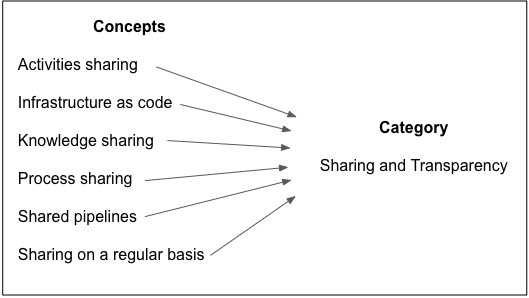
\includegraphics[width=0.5\textwidth]{fig1.png}
  \caption{Coding: Building Categories}
  \label{fig1}
\end{figure}


\subsection{Focus Group}
Focus group emerged as a research method in the social sciences in the 1950s
and is currently widely used, for example, in sociological studies, market
research, product planning, and system usability studies~\cite{shull2007guide}.
Morgan~\cite{morgan1996focus} defines focus group as a research technique that
collects data through group interaction on a specific topic determined by the
researcher.

According to F. Shull et al.~\cite{shull2007guide}, focus groups typically have
between three and twelve participants, are designed to obtain personal
perceptions of members of one or more groups involved in a defined area of
research interest and have as benefits the production of candid, often
insightful information, with a low cost and fast execution. These
characteristics make the focus group an adequate alternative to the purposes
of this evaluation. According to the authors, the discussion is guided and
facilitated by a researcher-moderator who follows a predefined structure of
questions.

We followed a structure similar to that performed by Lehtola et al.~\cite{requirementes_priorization_in_practice},
consequently, the focus group was conducted as follows: (1) the researcher-moderator served as
focus group facilitator providing participants with the discussion topics;
(2) at the beginning of each topic' discussion, the
questions were presented to participants who wrote their ideas and keywords in
post-it notes and (3) after that, the notes were placed on a white board and served
as a starting point for discussions on the respective topic in order to reach
conclusions about the respective question.
